%
\chapter{Discussion}
\label{ch:discussion}

The discussion chapter connects the results from the previous chapter to the theory, with focus on the aims of this work.
\brynjar{Brief summary of the aims.}
The overall aim of this work is to improve the performance of SEM EDS, which is done in three parts:
(1) to investigate how well the set-up is performing, (2) to investigate how well the acquisition parameters are chosen, and (3) to investigate bulk corrections for the quantification with open-source code.
The focus of this work for part (1) and (2) have been to find possible test metrics, describe them thoroughly in the theory chapter, and implement the metrics in code.
The metrics had to be tested on real data, which the reported results, but the main focus has been on the metrics themselves and not the acquisition of the data.
The focus for the data treatment in part (3) has been to implement SEM EDS bulk corrections in open-source code, as this is not available in the community at the time of writing.
Different approaches to the bulk corrections have been tested and are discussed in this chapter.
This chapter is built up as the results chapter, i.e. first discussing the qualitative analysis and the overview of the data, then the set-up performance metrics, then the acquisition parameters, and finally the bulk corrections.
At the end of the chapter, an additional section is added to discuss a possible test specimen, a critique of the SEM EDS standards, the flatness of specimen surfaces, and other possible metrics that were not done in this work.











\section{Qualitative analysis}
\label{discussion:qualitative_analysis}


% overview of the data
The overview spectra of GaAs and GaSb in \cref{fig:results:overviewGaSb_withArtifacts} and the voltage series in \cref{fig:results:GaAs_voltages,fig:results:GaSb_voltages} show that the acquired data is of varying quality.
The spectrum quality is affected by the beam energy and the amount of counts, which is revealed by looking at group A and B, being the voltage series of GaAs and GaSb.
The 30 kV and 15 kV spectra are in general of good quality with high counts, not too much noise, and clear peaks.
The spectra with the highest amount of counts have lower relative variations in the counts, seen as a more even plot of the blue 400 pA PT 1 spectrum compared to the 50 pA PT 1 spectrum in panel (a) of \cref{fig:results:overviewGaSb_withArtifacts}.
However, the amount of artifacts also increases with the amount of counts, exemplified by the previously mentioned spectra.
The 10 kV and 5 kV spectra have lower counts, as the beam current which was kept constant in the voltage series.
The lower counts were expected, and as seen in the voltage series figures, the 10 kV and 5 kV plots are visually of poorer quality.
With visually poorer quality, such as more noise and less clear peaks, the metrics and the quantification were expected to be worse.
In general the 5 kV and 10 kV spectra performed worse than the 15 kV and 30 kV spectra, which is discussed more in \cref{discussion:acquisition_parameters}.
As the 15 kV and 30 kV spectra performed better, these voltages were chosen for group C and D, where the goal was to investigate the effect of the beam current, beam energy, and process time.
These spectra all are assumed to have enough counts to be reasonably assessed with the metrics.


% linear vs log scale, artifacts
Qualitative analysis of EDS spectra are influenced by the choice of scale, i.e. linear or log scale.
AZtec has a default setting of a linear scale, with the option of a log scale.
The log scale is used in this work, as it highlights disturbances and makes the spectrum faster to assess.
This is especially true when a specimen contains trace elements, as the low peaks from the trace elements are more visible in the log scale.
The linear scale emphasizes the high peaks, making artifacts and disturbances less visible.
The coincidence peaks from the Sb L peaks visible in panel (a) of \cref{fig:results:overviewGaSb_withArtifacts} would be invisible in a linear scale, but the presence of coincidence counts lower the Fiori P/B metrics, tabulated in \cref{tab:results:fiori}.
The lower Fiori P/B ratio implies a poorer quality, as it is fewer counts in the Sb L$\alpha$ peak than it should be, and this could lead to a wrong quantification.
For GaSb spectra taken at 30 kV, the Fiori P/B ratio is similar at PT 1 and PT 6 with 50 pA beam current, and both these spectra have little coincidence counts.
In the 30 kV, 50 pA and PT 1 spectrum, where the coincidence rate is high, the Fiori P/B ratio is lower for Ga K$\alpha$, Sb L$\alpha$, and Sb L$\beta$.
In the same spectrum, the amount of coincidence counts from Ga L$\alpha$ does not increase, and the Fiori P/B ratio is similar to the other 30 kV spectra.
The log scale reveals the coincidence peaks, which is the source of the lower Fiori P/B ratio.
Another difference in the voltage series which would be hidden by a linear scale is the relative amount of counts in the background versus the peaks.
Below 2 keV the difference between the 30 kV and 15 kV spectra is small, but at increasing X-ray energy the 30 kV spectra have higher relative peak-to-background counts than the 15 kV spectra.
Looking at the Sb L$\alpha$ peak, which does not have an overvoltage issue, the background increase with a factor of around 2.5, while the peak increase with a factor of around 4.
The Fiori P/B ratios for the voltage series support this, as the general rule seems to be that a lower beam energy gives a lower Fiori P/B ratio.
If the spectra were only assessed with a linear scale, the difference in the background and peak counts would be less visible.
When assessing the quality of a spectrum, the log scale is therefore preferred.


% More on artifacts
% the C Ka peak. Contamination?
% no/little O Ka in GaAs.
Some artifacts seem to be affected by the amount of counts, and other artifacts are not.
As mentioned above, the coincidence events are affected by the amount of counts, giving both peaks and tailing counts.
The internal fluorescence Si peak is not affected by the amount of counts as the coincidence events are, and is present at similar low relative intensities in all spectra.
The carbon contamination in the form of a C K$\alpha$ peak is present in all spectra.
The absorption is high at low X-ray energies, but the C K$\alpha$ peak is present at similar relative intensities in all spectra.
However, the O K$\alpha$ peak is only present in the GaSb spectra, and not in the GaAs spectra.
The mass absorption coefficients for GaAs is twice as high at O K$\alpha$ than for GaSb, which could have been the reason for the O K$\alpha$ peak not being present in the GaAs spectra, but then the same should have been true for the C K$\alpha$ peak.
% GaAs: mu_rho(O_Ka) = 7k, mu_rho(C_Ka) = 24k
% GaSb: mu_rho(O_Ka) = 4k, mu_rho(C_Ka) = 11k
Thus, another explanation is needed for the absence of the O K$\alpha$ peak in the GaAs spectra.
It could be due to different contamination on the two specimens.
Another possibility is that the O K$\alpha$ peak is mislabeled, and is actually a Sb M-line.
This option is discussed in the second next paragraph.
\ton{Any other ideas?}


% absorption edge effects. suggest future work, splice
Similar absorption edge effects as observed in \cite{project_report} are present in the acquired spectra, where strong absorption edges at lower to medium energy influence the background intensities strongly.
This is illustrated well in \cref{fig:background_absorptionEdgeSi}, where the spectrum is overlaid with the mass absorption coefficient for Si.
The background intensity is reduced by the absorption edge, i.e. the intensity of the background is higher before the peak than after the peak.
This makes the background modelling more difficult, as the background is modelled with a polynomial function.
Lower accuracy in the background modelling could lead to worse quantification, as well as incorrect metrics discussed in this work.
One possible improvement to the background modelling is to use a spline function instead of a single polynomial function.


% Sb M-lines not in any table, but M is stated to be 0.733 keV at https://www.globalsino.com/EM/page4675.html
The last take-away from the qualitative analysis is that the HyperSpy database does not contain the Sb M-lines.
The GaSb spectra have a clear peak at what is assumed to be the Sb M$\eta$ peak around 0.42 keV, based on the qualitative analysis AZtec, as well as the absorption edge in Sb at 0.5 keV.
The energy of a line is located a few eV below the absorption edge.
The online book "Practical electron microscopy" by Y. Liao \cite{liao2006practical} lists a Sb M lines at 0.733 keV, but this is only visible in the spectra as a slight increase in counts and not a real peak.
The HyperSpy database and the X-ray data Booklet \cite{thompson_x-ray_2004} does not list any M-lines below Z=57.
A screenshot from the AZtec software, which identifies two Sb M-lines, one at 0.4 and a smaller at 0.7 keV, is shown in \cref{fig:discussion:AZtec_Mlines}.
The screenshot is of the spectrum with low energy resolution, and the 0.4 and 0.5 keV peak is overlapping, but the AZtec software clearly identifies the leftmost part of the merged peak as a Sb M-line.
This is an indication that the peak at 0.5 keV is not a Sb M-line, but rather that the O K$\alpha$ peak is labeled correctly.
The lack of the Sb M-lines in the HyperSpy database can be a source of error in the quantification, as the Sb M-lines are not included in the background modelling.
A solution to this is to slice off the spectrum before fitting the background so that unavailable lines are excluded from the background modelling.
This requires that the user visually inspect the lower energies thoroughly, and that the user is aware of the possibility of missing lines.
Another solution is to add the Sb M-lines to the HyperSpy database, which would require more research into M-lines of elements with Z lower than 57.

\begin{figure}[htbp]
    \centering
    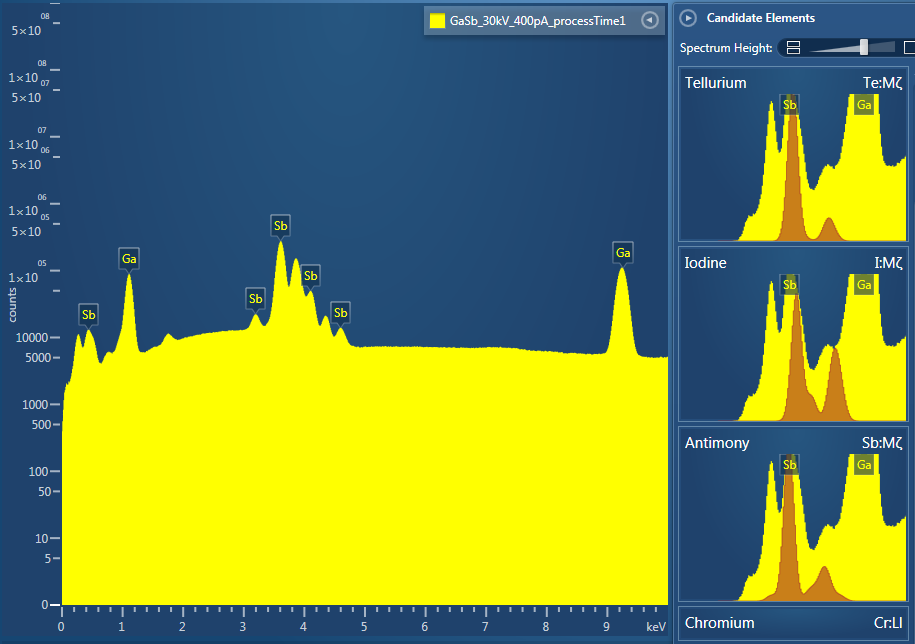
\includegraphics[width=0.95\linewidth]{figures/discussion/AZtec_Mlines.png}
    \caption{
        Screenshot from the AZtec software, showing the Sb M-lines identified at 0.4 and 0.7 keV.
        The right part of the screenshot show that tellurium and iodine match slightly better than antimony, but the L-lines present are definitely from antimony.
        }
    \label{fig:discussion:AZtec_Mlines}
\end{figure}

















\section{Set-up metrics}
\label{discussion:setup_metrics}













\section{Acquisition parameters}
\label{discussion:acquisition_parameters}














\section{Bulk corrections}
\label{discussion:bulk_corrections}














\section{Other discussions}
\label{discussion:other}

\subsection{Test specimen}
\label{discussion:other:test_specimen}

\subsection{SEM EDS standards}
\label{discussion:other:sem_eds_standards}

\subsection{Flatness of the specimen surface}
\label{discussion:other:flatness}

\subsection{Other metrics}
\label{discussion:other:other_metrics}




















%%%%%%%%%%%%%%%%%%%%%%%%%%%%%%%%%%%%%%%%%%%%%%%%%%%%%%%%%%%%%%%%%%%%%%%%%%%%%%%%%%%%%%%%%%%%%%%%%%%%%%%%%%%%%%%%%%%%%%%%%%%%%%%%%%%%%%%%%%%%%%%%%%%%%%%%%%%%%%%%%%%%%%%%%%%%%%%%%%%%%%%%%%%%%%%%%%%%%%%%%%%%%%%%%%%%%%%%%%%%%%%%%%%%%%%%%%%%%%%%%%%%%%%%%%%%%%%%%%%%%%%%%%%%

% This was in the old file:

%%%%%%%%%%%%%%%%%%%%%%%%%%%%%%%%%%%%%%%%%%%%%%%%%%%%%%%%%%%%%%%%%%%%%%%%%%%%%%%%%%%%%%%%%%%%%%%%%%%%%%%%%%%%%%%%%%%%%%%%%%%%%%%%%%%%%%%%%%%%%%%%%%%%%%%%%%%%%%%%%%%%%%%%%%%%%%%%%%%%%%%%%%%%%%%%%%%%%%%%%%%%%%%%%%%%%%%%%%%%%%%%%%%%%%%%%%%%%%%%%%%%%%%%%%%%%%%%%%%%%%%%%%%%

% Flatness of the specimen surface
% check out: Newbury and Ritchie 2013, Quantitative SEM/EDS, Step 1: What Constitutes a Sufficiently Flat Specimen?
% https://www.cambridge.org/core/services/aop-cambridge-core/content/view/E9E18A67EED08A3A7F23C4559F81DE93/S1431927613008210a.pdf/quantitative-semeds-step-1-what-constitutes-a-sufficiently-flat-specimen.pdf





% \section{Regarding the ISO 15632 standard}
% \label{theory:eds_performance:iso15632}

% BAM (Federal Institute for Materials Research and Testing) has a test sample for SEM EDS with a accompanying software, which satisfies the ISO 15632 standard.
% However, the price per 28.02.2023 for this sample (EDS TM002) is 334 EUR and 335 EUR for the software.
% A full test in accordance with the ISO standard could probably be done with a cheaper sample and a Jupyter Notebook, where the user would see all the steps and the results.
% This has not been a main focus in this work, but some parameters in the ISO standard are covered in this work.

% \url{https://webshop.bam.de/webshop_de/eds-tm002.html}

% paper at \url{https://www.cambridge.org/core/services/aop-cambridge-core/content/view/17A1D769BB6B9B76B5AC815911FAE7FD/S1431927613008271a.pdf/check-and-specification-of-the-performance-of-eds-systems-attached-to-the-sem-by-means-of-a-new-test-material-eds-tm002-and-an-updated-evaluation-software-package-eds-spectrometer-test-version-3-4.pdf}





% TODO: energy resolution. the older xmax info claims high energy resolution and high cps. The x-max-N datasheet lists resolution with cps, which is nicer. Progress.




% \section{Qualitative analysis}
% \label{method:qualitative_analysis}

% See Annex A in ISO 22309. Also make a notebook, which can be shared with HyperSpy people.
% Show the use of find_peak_ohaver, referring to O'Haver's paper, with different settings.
% Also show nice plotly plots, eventually plt with plotting all lines in HS for the element.
% And maybe also fitting, where the area is shown to see if any added elements are 0.
% Can refer to autoID, and it's flaws.

% Rule for what a peak is? See eg Annex A in ISO 22309: I > (BG + 3 x sqrt(BG)), wher BG is mean of BG (probably at the given energy)

% \brynjar{ISO 22309: "typically a value of 30 eV can be critical; peaks separated by more than this figure should not be confused by either automatic or manual identification procedures."}





% \subsection{Calibration}
% \label{method:calibration}

% For some reason, it works better to calibrate the offset and then the scale/dispersion.
% HyperSpy allows for calibration of offset, scale or energy resolution, but only one at a time.
% The procedure used was: calibrate offset, calibrate scale, recaliabrate offset, and recalibrate scale.
% After the recalibration, the difference was compared to the first calibration, and if the change was more than 5\%, the calibration was repeated.
% By default, the HyperSpy calibration uses all alpha lines.
% It is possible to specify certain lines to calibrate on, but this yeilded the same or worse results as using all alpha lines.
% \brynjar{The stuff above is more discussion, at least the last sentence.}






% \subsection{The requirements for a standard material}
% \label{theory:eds_performance:standard_material}
% smt about the standard materials available \dots
% what we want in the spectrum \dots
% candidates \dots







% \subsection{Other tests - not used in this work}
% \label{theory:eds_performance:other}

% \brynjar{TODO from Ton: "if not used, do not include them. But consider to use them in discussion leading to concrete future work (last chapter)"}

% Other test are described in the literature, but they were not used in this work.
% Some of them is mentioned here, either because they are interesting but not possible, because they are not relevant enough, or because they could be relevant in future works.

% \subsubsection*{Linearity and stability}
% In Goldstein \cite[p. 232]{goldstein_scanning_2018} it is stated that the two most important tests for an EDS detector are linearity and stability.
% This is stated in the section about what to look for when buying a detector.
% The reason for not including these two test in the work is mainly their dependence on a way to measure the probe current, which e.g. can be done with a Faraday cup.
% Such tests could be used in the future and are therefore briefly described here.
% Linearity of the detector is that the number of X-rays measured is proportional to the number of X-rays generated.
% Stability is that the detector resolution and the peak positions does not change significantly with different probe currents.
% Both tests require multiple spectra of the same sample with different probe currents.
% The ISO 22309 standard on quantification of EDS spectra \cite{iso_quantification_22309} also mentions these two tests.

% % \brynjar{ISO 22309: "Whatever type of detector is being used, the count rate capabilities of the system should be checked by
% %     comparing a spectrum obtained at a count rate below 2 000 counts/s with a spectrum obtained at the highest
% %     count rate to be used, to look for peak shift and pile-up distortion that might affect relative peak heights. A
% %     minimum of two checks on beam stability, using a Faraday cup, or a known reference specimen, should be
% %     made prior to and following the analysis."}

% % TODO : kan jeg gjøre de med beam current???



% \subsubsection*{Peak shape}

% Deviations of peak shapes can be used to identify problems with the detector or the qualitative analysis.
% Peak shapes are used in Egerton and Chengs work to identify incomplete charge collection, but this is a lesser concern in modern SDDs.
% Peak shapes deviating from a Gaussian shape, which is not due to detector issues, are probably due to misidentification where a minor peak is not correctly identified.
% The overlapping peak has the counts from both peaks, and the shape will be skewed.
% Assessing the peak shape with numbers is not straightforward, but the FWHM/FWTM can be used to compare the peak shape of different spectra.
% This requires the peaks to be standing alone, without any overlap.
% As this is not always the case, and that the metric is not too useful, it is not used in this work.
% However, an analyst should be aware of the peak shape, as it can be useful if a skewed peak is found and lacking a clear explanation.

% Overlapping peaks, ASTM 1508:
% "9.2.5 Next look for peak overlaps. If (1) a peak is displaced
% relative to its marker, (2) relative intensities are wrong, or (3)
% there is a distortion in the peak shape, then there is an
% overlapping element. All three conditions will be present in an
% overlap situation."


% \subsubsection*{Shadowing}
% \brynjar{From ISO 15632: "In many cases the specific geometry of the EDS detector at a particular SEM/EPMA chamber can result in a reduction of the net active sensor area as expected after subtraction of shadowing area caused by the window grid. For example, a falsely mounted collimator, electron trap or shadowing by other parts in the SEM chamber can reduce additionally the illumination of the detector with X-rays. A practical procedure how to determine experimentally the effective area of an EDS detector and under which conditions are described in Reference [5]."}
% % [5] Procop M., Hodoroaba V.-D., Terborg R., Berger D., Determination of the Effective
% % Detector Area of an Energy-Dispersive X-Ray Spectrometer at the Scanning Electron
% % Microscope Using Experimental and Theoretical X-Ray Emission Yields, Microsc. Microanal.,
% % 22 (2016), pp. 1360-1368
% % Shadowing



% \subsubsection*{Energy dependence of instrumental detection efficiency - K/L ratio}
% \brynjar{ISO 15632: "The minimum specification for the energy dependence of the instrumental detection efficiency shall be
%     the intensity ratio of a low energy line and a high energy line in the characteristic X-ray spectrum of a
%     given material. This ratio shall be given as the net peak area of the L series lines divided by the net peak
%     area of K$\alpha$ series lines in the spectrum of a pure nickel or copper specimen, excited by a 20 keV electron
%     beam perpendicular to the specimen surface and collected by the detector at a take-off angle of 35 degrees. The
%     specimens to be used, the measurement conditions, the calculation of L/K ratio and its conversion for
%     TOA not equal 35 degrees are given in Annex B. \dots These measures are only appropriate for a detector thick enough to absorb at least 95 % of the incident
%     X-ray energy at 8 keV."}


% \subsubsection*{Optimal WD}
% \url{https://www.cstl.nist.gov/div837/837.02/epq/dtsa2/FaultsFoiblesEDS.pdf}
% % \brynjar{En geometrigreie. Er det forskjellig for ulike materialer? Passer under acquisition params}